% tikz in document class for perceptron picture
\documentclass[12pt, tikz, letterpaper]{article}
\usepackage[utf8]{inputenc} %document endcoding
\title{CAP 6619 Deep Learning Homework 1}
\author{John Hancock}

% for picture of perceptron
\usepackage{tikz}
   \usetikzlibrary{positioning}

\tikzset{basic/.style={draw,fill=blue!20,text width=1em,text badly centered}}
\tikzset{input/.style={basic,circle}}
\tikzset{weights/.style={basic,rectangle}}
\tikzset{functions/.style={basic,circle,fill=blue!10}}

% for block quote
\usepackage{etoolbox}

\begin{document}
\maketitle
\section{Introduction}
This document contains our answers to the questions in the first homework 
assignment of CAP 6619: Deep Learning, taught by Dr. Xingquan Zhu at Florida
Atlantic University in the Fall of 2018.

Dr. Zhu is the author of the questions and tasks we answer and do in this 
document. We find the original document specifying this first homework 
assignment in \cite{homework1}. 

\section{Question 1}

Homework one begins with a task and two questions

\begin{quote}
Please show the perceptron structure and explain the function of each component
[0.5 pt]. What is the purpose of using training examples in a neural network? Given property weight
values, what is expected output vs. actual output of an example? [0.5 pt] 
\cite{homework1}
\end{quote} 

\subsection{Perceptron Structure}
Dr. Zhu gives the perceptron structure in \cite{perceptronlecture}. On slide
number 8 Dr. Zhu gives a digram.  We copy the \LaTeX code from 
\cite{perceptronpic} to create the digram in \ref{fig:perceptron} that is 
equivalent to the one Dr. Zhu gives in \cite{perceptronlecture}.
\begin{figure}[h]
\label{fig:perceptron}
\caption{Perceptron}
 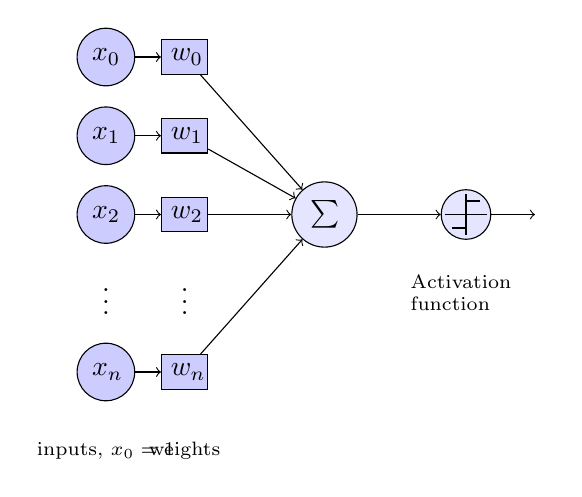
\begin{tikzpicture}
        \node[functions] (center) {};
        \node[below of=center,font=\scriptsize,text width=4em] {Activation function};
        \draw[thick] (0.5em,0.5em) -- (0,0.5em) -- (0,-0.5em) -- (-0.5em,-0.5em);
        \draw (0em,0.75em) -- (0em,-0.75em);
        \draw (0.75em,0em) -- (-0.75em,0em);
        \node[right of=center] (right) {};
            \path[draw,->] (center) -- (right);
        \node[functions,left=3em of center] (left) {$\sum$};
            \path[draw,->] (left) -- (center);
        \node[weights,left=3em of left] (2) {$w_2$} -- (2) node[input,left of=2] (l2) {$x_2$};
            \path[draw,->] (l2) -- (2);
            \path[draw,->] (2) -- (left);
        \node[below of=2] (dots) {$\vdots$} -- (dots) node[left of=dots] (ldots) {$\vdots$};
        \node[weights,below of=dots] (n) {$w_n$} -- (n) node[input,left of=n] (ln) {$x_n$};
            \path[draw,->] (ln) -- (n);
            \path[draw,->] (n) -- (left);
        \node[weights,above of=2] (1) {$w_1$} -- (1) node[input,left of=1] (l1) {$x_1$};
            \path[draw,->] (l1) -- (1);
            \path[draw,->] (1) -- (left);
        \node[weights,above of=1] (0) {$w_0$} -- (0) node[input,left of=0] (l0) {$x_0$};
            \path[draw,->] (l0) -- (0);
            \path[draw,->] (0) -- (left);
        \node[below of=ln,font=\scriptsize] {inputs, $x_0=1$};
        \node[below of=n,font=\scriptsize] {weights};
    \end{tikzpicture}
\end{figure}
\begin{thebibliography}{9}
% we use ACM citation format: 
% https://www.acm.org/publications/authors/reference-formatting
% Note: URL citations end with a '.' if and only if the URL ends with '/'.

\bibitem{homework1}
Xingquan Zhu. 2018. Homework 1. (September 2018). Retrieved September 7, 2018
from \\\texttt{https://canvas.fau.edu/files/14059715/download?download\_frd}

\bibitem{perceptronlecture}
Xingquan Zhu. 2018. Perceptron Architecture and Learning. (August 2018). 
Retrieved September 8, 2018 from \\\texttt{https://canvas.fau.edu/courses/50073/files/folder/Lectures?preview=14020569}

\bibitem{perceptronpic}
tex.stackexchange.com user m0nhawk. 2 of 2. (26 March 2013). Retrieved September
9, 2018 from \\\texttt{https://tex.stackexchange.com/revisions/104376/2}

\end{thebibliography}

\end{document}
